%%%%%%%%%%%%%%%%%%%%%%%%%%%%%%%%%%%%%%%%%%%%%%%%%%%%%%%%%%%%%%%%%%%%%%%%%%%
%% This file is part of the book
%%
%% Algorithmic Graph Theory
%% http://code.google.com/p/graph-theory-algorithms-book/
%%
%% Copyright (C) 2009--2011 Minh Van Nguyen <nguyenminh2@gmail.com>
%%
%% See the file COPYING for copying conditions.
%%%%%%%%%%%%%%%%%%%%%%%%%%%%%%%%%%%%%%%%%%%%%%%%%%%%%%%%%%%%%%%%%%%%%%%%%%%

\documentclass{article}

\usepackage{tikz}
\usetikzlibrary{external}
\tikzexternalize{von-Neumann-neighborhood}

\begin{document}

\begin{figure}[!htbp]
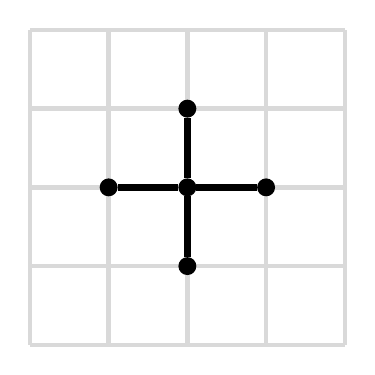
\begin{tikzpicture}
[blackFilled/.style={shape=circle,fill=black,inner sep=2pt,draw,thick},%
  darkLine/.style={line width=2.5pt},%
  lightLine/.style={-,ultra thick,color=gray!30}]
%% set up the grid
\foreach \xstart/\xend/\y in {0/4/0, 0/4/1, 0/4/2, 0/4/3, 0/4/4}
{
  \draw[lightLine] (\xstart,\y) -- (\xend,\y);
  \draw[lightLine] (\y,\xstart) -- (\y,\xend);
}
%% draw the nodes
\foreach \nodename/\x/\y in {center/2/2, north/2/3, south/2/1,
  east/3/2, west/1/2}
{
  \node (\nodename) at (\x,\y) [blackFilled] {};
}
%% draw the edges
\foreach \u/\v in {center/north, center/south, center/east, center/west}
{
  \draw[darkLine] (\u) -- (\v);
}
\end{tikzpicture}
\end{figure}

\end{document}
